   \newpage
   \section{Systemüberblick und Systemarchitektur}
   Im Folgenden soll ein Überblick der verwendeten Systemkomponenten gegen werden. In Abbildung 2 ist der generelle Ablauf der Kommunikation zwischen den Komponenten dargestellt. Die emotionale Erregung des Nutzers soll über zwei Sensoren gemessen werden. Zum einen erfolgt eine Messung des elektrischen Widerstandes der Haut über einen Galvanic Skin Sensor. Der Galvanic Skin Sensor kommuniziert über eine Bluetooth-Verbindung mit einem Arduino Shield. Das Arduino Shield wiederum ist via Bluetooth mit dem Smartphone des Nutzers verbunden. Der zweite Sensor ermöglicht die Registrierung der Hirnströme und wird als  Elektroenzephalografie, kurz EEG, bezeichnet. Der EEG-Sensor kommuniziert ebenfalls über das Bluetooth-Protokoll mit dem Smartphone. Im Smartphone werden die vom Nutzer gewonnenen Daten ausgewertet und verständlich dargestellt. Messergebnisse können zum einen lokal in einer Datenbank abgelegt werden oder auch mit anderen Freunden auf einer Social Media Plattform geteilt werden.
   	\begin{figure}[ht!]
		\begin{center}
			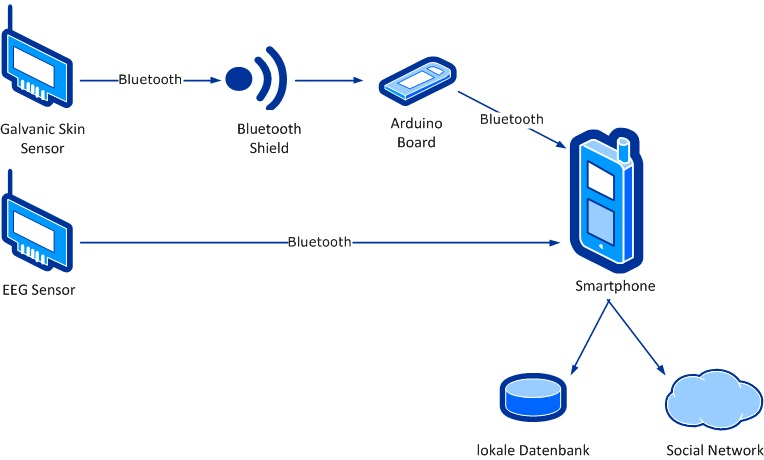
\includegraphics[width=0.9\textwidth]{systemarchitektur_01.jpg}
		\end{center}
		\caption[Systemarchitektur]{Systemarchitektur}
		\label{fig:system1}
	\end{figure}	
